\subsection{Análise DRX}

\begin{frame}{Material e métodos}{Análise dados DRX}

	\tikzset{block/.style={rectangle, draw, text width=15em, rounded corners, minimum width=3.5cm}}
	\tikzset{title/.style={rectangle, text centered, text width=15em, minimum width=3.5cm, font=\bfseries}}
	\tikzset{figure/.style={rectangle, text width=20em, minimum width=3.5cm}}
	\tikzset{line/.style={draw, -latex}}


	\scalebox{0.55}{
		\begin{tikzpicture}
			\node[block,text centered](raw){Dados brutos};
			\node[block, below=1cm of raw](Gauss){Ajuste dos picos por função de Gauss\footnotemark[1]:\\
				$I = I_0 \exp{\left[-\left(\frac{2\theta - 2\theta_0}{w}\right)^2\right]}$\alert{ + bck}};
			\node[block, left=1cm of Gauss](integral){Integração dos picos:\\
				$A = \int\limits_{-\infty}^{\infty} I_0 \exp{\left[-\left(\frac{2\theta - 2\theta_0}{w}\right)^2\right]} d\theta =$\\
				$= I_0|w|\sqrt{\pi}$};
			\node[block, below=1cm of integral](Cullity){Cálculo de $f^\gamma$ pela comparação com intensidades calculadas\footnotemark[2]:\\
				$f^\gamma = 1 - f^\alpha = \frac{\sum A_{hkl}^\gamma/R_{hkl}^\gamma}{\sum A_{hkl}^\alpha/R_{hkl}^\alpha + \sum A_{hkl}^\gamma/R_{hkl}^\gamma}$};
			\node[block, right=1cm of Gauss](Bragg){Lei de Bragg $\rightarrow$ converter $2\theta_0$ para $a_{TP}^\gamma$};
			\node[block, below=1cm of Bragg](correction){Experimentos \textit{in situ} foram feitos na temp. TP $\rightarrow$ transformar $a_{TP}^\gamma$ para $a_{300K}^\gamma$ usando eq. de expansão do reticulado\footnotemark[3]:\\
				$\frac{\Delta L^\gamma}{L_0^\gamma} = B_\gamma T + B_\gamma \Theta_D^\gamma \left[ \exp{\left( -\frac{T}{\Theta_D^\gamma} \right)}\right]$\\
				em que $B_\gamma=24,8\times 10^{-1} K^{-1}$ e $\Theta_D^\gamma=280 K$};
			\node[block, below=1cm of correction](Dyson){Computar teor de carbono utilizando relação entre $a^\gamma$ e $\%w_C^\gamma$ de Dyson e Holmes\footnotemark[4]:\\
				$a^\gamma = 3,5780 + 3,30\cdot10^{-2} \%w_C^\gamma + 9,5\cdot10^{-4} \%w_{Mn}^\gamma + 1,5\cdot10^{-3} \%w_{Cu}^\gamma$};
			\node[figure, below=0.5cm of Gauss]{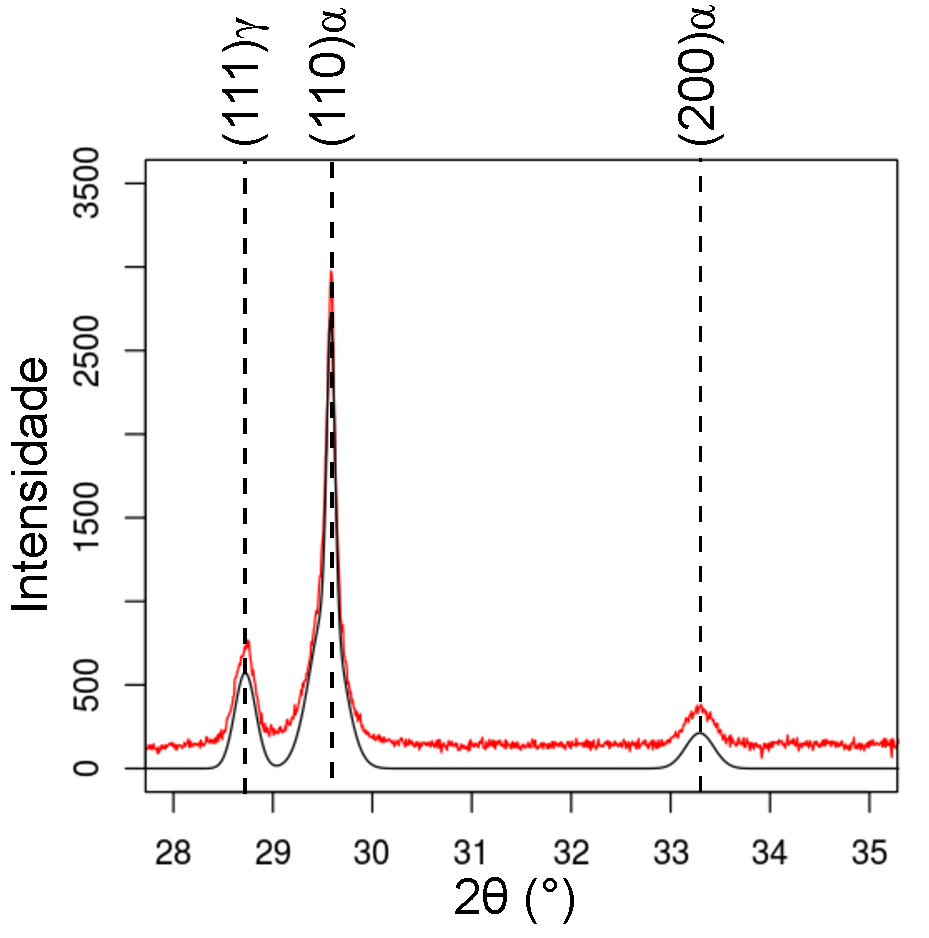
\includegraphics[width=20em]{img/peak_fitting}};
			\node[title, above=0.5cm of integral]{Cálculo das frações volumétricas de $\alpha$ e $\gamma$};
			\node[title, above=0.5cm of Bragg]{Cálculo do teor de carbono em $\gamma$};

			\path[line](raw) -- (Gauss);
			\path[line](Gauss) -- (integral);
			\path[line](integral) -- (Cullity);
			\path[line](Gauss) -- (Bragg);
			\path[line](Bragg) -- (correction);
			\path[line](correction) -- (Dyson);
		\end{tikzpicture}
	}
	\footnotetext[1]{Babu SS, Specht ED, David SA, Karapetrova E, Zschack P, Peet M, Bhadeshia HKDH. Metall Mater Trans A 2005;36:3281.}
	\footnotetext[2]{Stock S, Cullity B. Elements of X-ray diffracion. Prentice Hall, New Jersey, 2001}
	\footnotetext[3]{van Bohemen SMC. Scr Mater 2013;69:315.}
	\footnotetext[4]{Dyson DJ, Holmes B. J Iron Steel Inst 1970;208:469.}

\end{frame}